\documentclass[12pt]{article}

\usepackage[onlytext]{MinionPro}
\usepackage{microtype}                                                          % Better looking documents "typographical perfection"

\usepackage[left=3cm, right=3cm]{geometry}		                                % Margins left and right
\usepackage{hyperref}                                                           % Clickable table of contents in PDFs
\usepackage{datetime}                                                           % Currenttime
\usepackage[titletoc,title]{appendix}                                           % Appendices in table of contents

\usepackage{graphicx}                                                           % Include figures
\usepackage{float}                                                              % Better float options: H(ere)
\usepackage[most]{tcolorbox}                                                    % Breakable box for digressions

\usepackage{physics}                                                            % Physics typesetting: bra-ket
\usepackage{mathtools}                                                          % for the custom command \set and
                                                                                % package amsmath: \tag
\usepackage{xparse}                                                             % for the custom command \set
\usepackage{mathrsfs}                                                           % \mathsrc
\usepackage{amssymb}                                                            % \mathbb
\usepackage{amsthm}                                                             % \qedhere
\usepackage{interval}

\numberwithin{equation}{section}                                                % Equations are numbered per section
\numberwithin{figure}{section}                                                  % Figures are numbered per subsection

\setlength{\parindent}{0in}                                                     % No indentation for every paragraph
  % Packages for this project
% % % Special notations for sets of numbers
\newcommand{\N}{\mathbb{N}}                                                     % Natural numbers
\newcommand{\R}{\mathbb{R}}                                                     % Real numbers
\newcommand{\C}{\mathbb{C}}                                                     % Complex numbers
\newcommand{\F}{\mathbb{F}}                                                     % General field, R or C

% % % Special notations for groups
\DeclareMathOperator{\GLg}{GL}                                                  % General linear group
\DeclareMathOperator{\SLg}{SL}                                                  % Special linear group
\DeclareMathOperator{\Og}{O}                                                    % Orthogonal group
\DeclareMathOperator{\SOg}{SO}                                                  % Special orthogonal group
\DeclareMathOperator{\Ug}{U}                                                    % Unitary group
\DeclareMathOperator{\SUg}{SU}                                                  % Special unitary group
\DeclareMathOperator{\Aut}{Aut}                                                 % The automorphism group

% % % Other math operators
\DeclareMathOperator{\id}{id}                                                   % Identity function
\DeclareMathOperator{\diag}{diag}                                               % Diagonal matrix


% Create a custom command for set notation
%
\DeclarePairedDelimiterX{\set}[1]{\{}{\}}{\setargs{#1}}
\NewDocumentCommand{\setargs}{>{\SplitArgument{1}{;}}m}
{\setargsaux#1}
\NewDocumentCommand{\setargsaux}{mm}
{\IfNoValueTF{#2}{#1} {#1\,\delimsize|\,\mathopen{}#2}}%{#1\:;\:#2}
  % Custom commands for this project


\title{Mathematics}
\author{Laurent Lemmens \\ GQCG}
\date{\today \hspace{6pt} \currenttime}


\begin{document}

\maketitle

% % % ABSTRACT AND TABLE OF CONTENTS

% Abstract
\begin{abstract} \noindent  % enters inside the abstract are not rendered as line breaks in the .pdf-file
    These notes serve as a summary of mathematics I have thorougly studied.
\end{abstract}

% Line after abstract
\begin{center}
    \line(1,0){250}
\end{center}

% Table of contents
\tableofcontents
\newpage


% % % MAIN TEXT % % %
\section{Modern algebra}
    Modern algebra \cite{joyce2008}, or abstract algebra, is the mathematical branch that studies sets and associated operations (algebraic structures) and relations between them.

    \subsection{Functions - relations between sets}
    \subsubsection{Sets}
        Modern algebra starts from the notion of a set. A set $S$ is a collection of elements:
        \begin{equation}
            S = \set{s_1, s_2, \dots, s_n} \thinspace .
        \end{equation}
        Some examples of sets are the set of natural numbers $\N$, the set of real numbers $\R$, the set of complex numbers $\C$. We can also have smaller sets, for example
        \begin{equation}
            S = \set{0, 1} \thinspace ,
        \end{equation}
        being the set of the numbers $0$ and $1$. Sets don't necessarily have to contain only numbers. We can, for example, collect all invertible $n \times n$-matrices in a set:
        \begin{equation}
            \GLg(n, \mathbb{R}) = \set{A \in \mathbb{R}^{n \times n} ; \text{$A$ is invertible}} \thinspace ,
        \end{equation}
        in which the symbol $\GLg$ has to do with `general linear', but more on that when we encounter the general linear group. \\

        The previous examples are all concrete (i.e. not abstract) examples of sets. Now say we have a mathematical object, called $E$ (we haven't specified anything about it), we can say that
        \begin{equation}
            G = \set{E}
        \end{equation}
        is also a set, but in a more abstract sense than the previous examples. We can enlarge this set by adding the elements $C_2, \sigma_v$ and $\sigma_v'$, to end up with
        \begin{equation}
            G = \set{E, C_2, \sigma_v, \sigma_v'} \thinspace ,
        \end{equation}
        in which we still haven't specified anything about the nature of its elements, but in mathematics that is perfectly fine. \\

    \subsubsection{Functions - introduction}
        Naturally, if we have two different sets, we would like to be able to define relations between their elements. This is exactly what a function does. A function (or map, mapping, these are all synonyms) is a relation between two sets $X$ and $Y$:
        \begin{equation} \label{eq:def_function}
            f: X \rightarrow Y: x \mapsto y = f(x) ,
        \end{equation}
        subject to the important condition that every input $x \in X$ is related to exactly one output $y \in Y$. We would read the definition in equation (\ref{eq:def_function}) as follows: $f$ is a function from the set $X$ to the set $Y$, in which every $x \in X$ is related to a $y \in Y$, which we call $f(x)$. \\

        We give special names to the sets $X$ and $Y$, depending on which role they play in the function. The set $X$ is called the domain of the function: it is the set of all inputs for the function. The set $Y$ is then called the function's codomain: it is the set of values that \emph{could} occur as output values for the function. We can then define another set, $Z$, which is called the image of the function: it is the set of \emph{actual} values for the outputs. A visual clarification of the terms can be found in Figure \ref{fig:functions}. \\
        \begin{figure}[H] \centering
            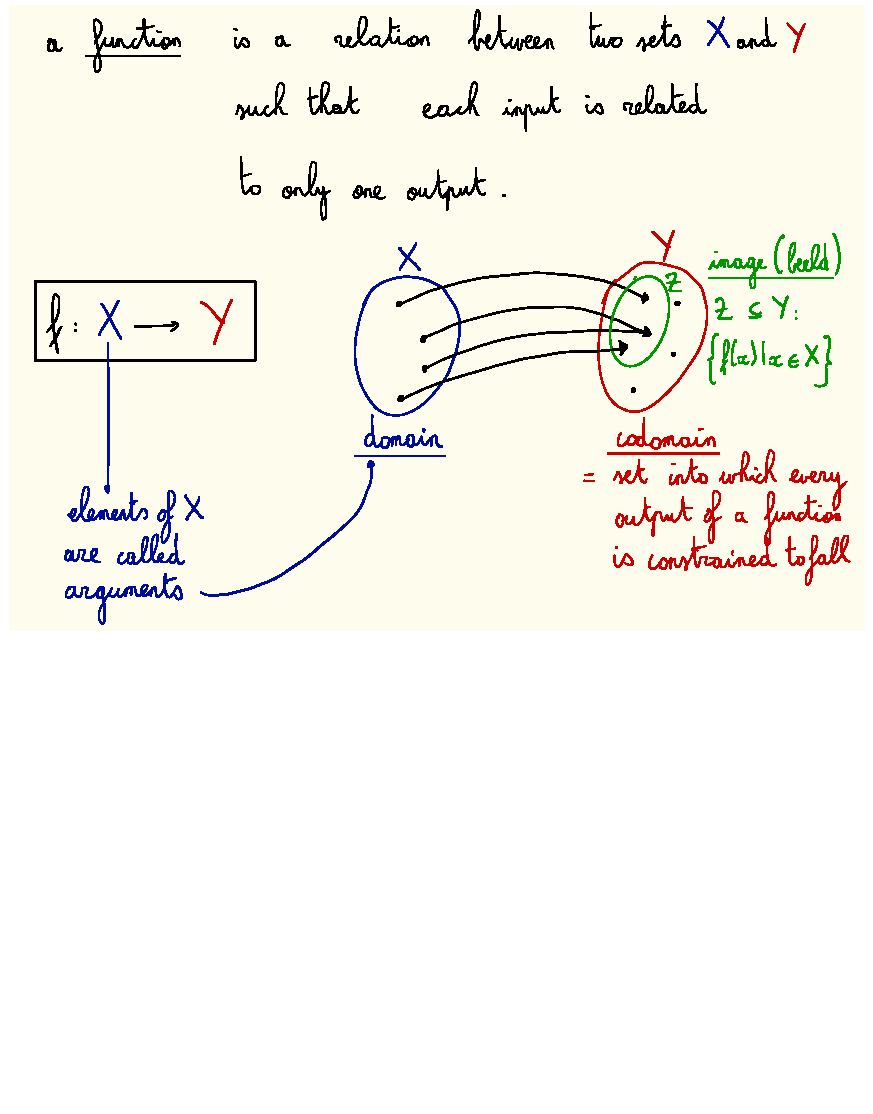
\includegraphics{images/functions}
            \caption{The definition of a function, and a visual clarification of the terms domain, codomain and image. The domain is the set of input values, the codomain is the set of possible output values, and the images is the set of actual output values.}
            \label{fig:functions}
        \end{figure}

        An example of a function could be:
        \begin{equation}
            f: \R \rightarrow \R: x \mapsto f(x) = x^2 + 2
        \end{equation}
        Its domain is $\R$, and its codomain is also $\R$. Here, we can also see the difference between the codomain and the image. The codomain of this function is defined to be $\R$, but its image $[2, +\infty[$. Another example is shown in Figure \ref{fig:function_color}.
        \begin{figure}[H] \centering
            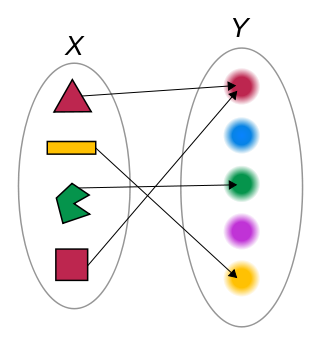
\includegraphics[scale=0.4]{images/function_color}
            \caption{An example of a function that maps an object to its color.}
            \label{fig:function_color}
        \end{figure}
        The reason why this is a function is because every input element of the set $X$, being shapes in a certain color, is related to its color, represented as elements of the set $Y$. In this case, $Y$, the codomain is the set of colors depicted as elements of $Y$, and the range is the set of colors red, green and yellow. \\

        We have seen some examples of functions already, but what are some examples of non-functions? There are actually two requirements to the definition of a function:
        \begin{enumerate}
            \item Every input (element of the domain) has to be related to an output (element of the codomain)
            \item No two outputs (elements of the codomain) may be related to the same input (element of the domain)
        \end{enumerate}
        With these two criteria in mind, it is possible to come up with many examples of relations between two sets that are not functions, for example those shown in Figure \ref{fig:non_functions}.
        \begin{figure}[H] \centering
            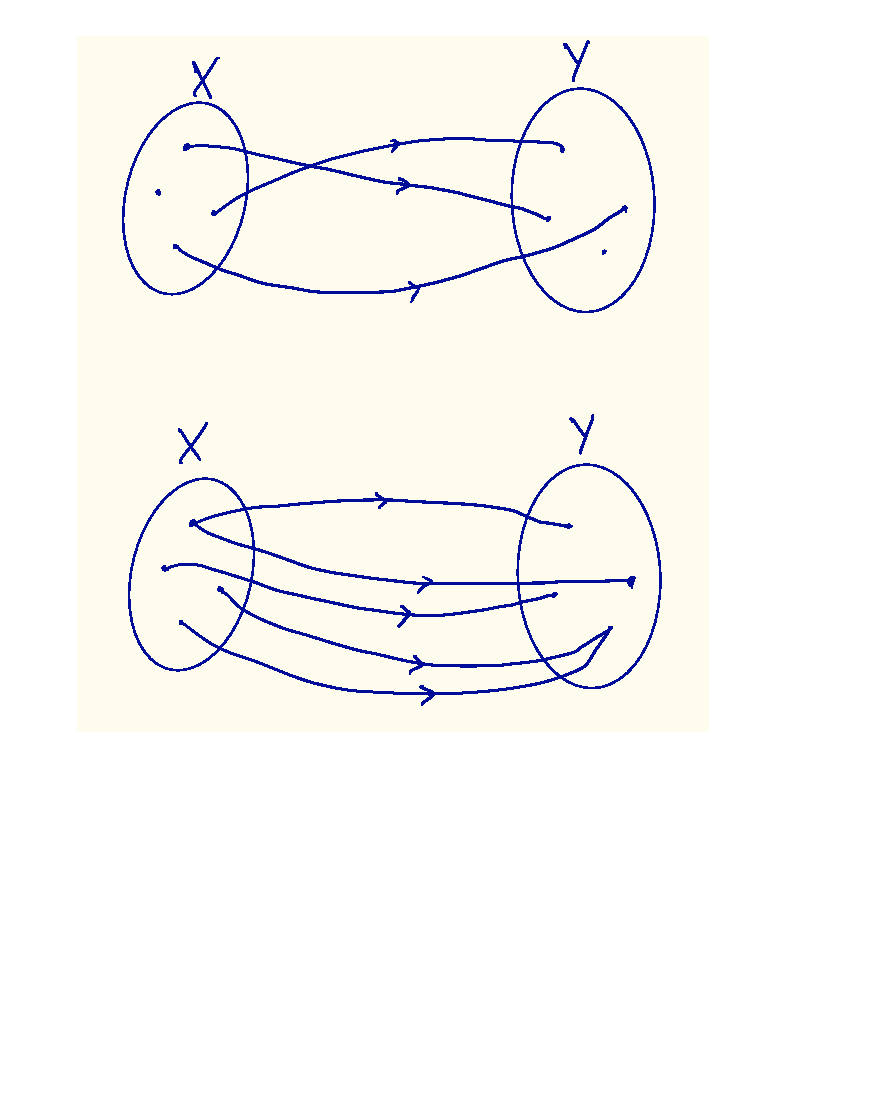
\includegraphics{images/non_functions}
            \caption{Two examples of non-functions. The first relation between $X$ and $Y$ is not a function, because not every element of $X$ is related to an element of $Y$. The second figure is not a function because there is an element of $X$ related to two elements of $Y$.}
            \label{fig:non_functions}
        \end{figure}

    \subsubsection{Classification of functions}
        By now, we have seen some examples of functions. In order to classify functions, we will introduce the terms surjection, injection, and bijection. For a visual overview of the terms, see Figure \ref{fig:sur_in_bi}. \\

        A function is called surjective (or: onto), if every element of its codomain is mapped to. \emph{Sur} means `above', which relates to the fact that the function's codomain is completely covered. Its definition can be written as follows: a function $f$ is said to be surjective if
        \begin{equation}
            f: X \rightarrow Y: \forall y \in Y: \exists x \in X: f(x) = y \thinspace .
        \end{equation}

        A function is called injective (or: one-to-one) if no element of its codomain is mapped to twice. Mathematically, we would write: $f$ is an injective function if
        \begin{equation}
            f: X \rightarrow Y: \forall a, b \in X: f(a) = f(b) \Rightarrow a = b \thinspace .
        \end{equation}

        A function is called bijective (or: one-to-one and onto, a one-to-one correspondence), if it is both injective and surjective: every element of the codomain is mapped to by exactly one element of the domain. \\

        The identity function on a set $S$ is the function:
        \begin{equation}
            \id_S: S \rightarrow S: \id_S(s) = s \thinspace .
        \end{equation}

        \begin{figure}[H] \centering
            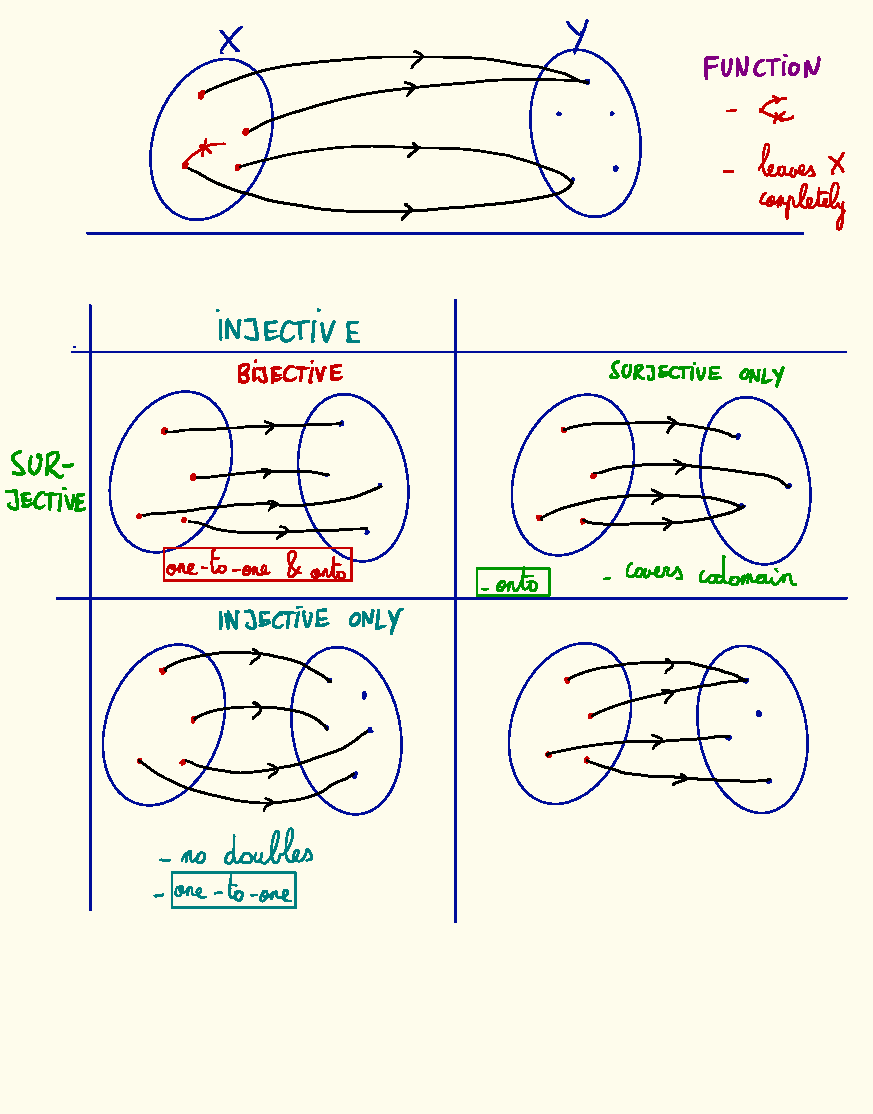
\includegraphics{images/sur_in_bi}
            \caption{A visual scheme of the terms surjective, injective and bijective.}
            \label{fig:sur_in_bi}
        \end{figure}

        Given Figure \ref{fig:sur_in_bi}, we can already see examples of surjective and injective functions. In Figure \ref{fig:function_color}, we can see an example of a function that is not surjective (not every color is mapped to), nor injective (the color red is mapped to twice). \\

    \subsubsection{More types of functions}
        An operation is a special kind of function. It is a function
        \begin{equation}
            \omega: X^n \rightarrow X \thinspace ,
        \end{equation}
        which takes $n$ elements from the set $X$ as input, and relates that combination to the set $X$ itself. \\

        We know many operations, for example number addition, which takes two numbers as input and relates that combination to another number. Number multiplication is another example of a binary operation: we take two numbers, whose product is another number. The set $X$ is not confined to be a set of numbers. If we take, for example, set of $n \times n$ matrices, then matrix multiplication is an example of a binary operation. \\


    \subsection{Algebraic structures}
    Algebraic structures are a combination of a set, together with one or more operations, satisfying a list of axioms.

    \subsubsection{The mathematical definition of a group} \label{sec:group_def}
        A group has a mathematical definition. It is a set $G$\footnote{We often use the same symbol to denote the set of group elements and the actual group. I don't think there is anything wrong with this, as the distinction is most often clear from the context.} with elements $G=\set{g_1, g_2, \dots, g_n}$, together with an operation $\cdot$ (which is often called the group multiplication), meeting the following axioms:
        \begin{enumerate}
            \item closedness
            \begin{equation}
                \forall g_1, g_2 \in G: g_1 \cdot g_2 \in G
            \end{equation}

            \item associativity
            \begin{equation}
                \forall g_1, g_2, g_3 \in G: g_1 \cdot (g_2 \cdot g_3) = (g_1 \cdot g_2) \cdot g_3
            \end{equation}

            \item identity element
            \begin{equation} \label{eq:group_id}
                \exists! \thinspace e \in G: \forall g \in G: e \cdot g = g \cdot e = g
            \end{equation}

            \item inverses
            \begin{equation}
                \forall g \in G: \exists! \thinspace g^{-1} \in G: g \cdot g^{-1} = g^{-1} \cdot g = e
            \end{equation}
        \end{enumerate}
        If the axiom
        \begin{enumerate}
            \setcounter{enumi}{4}
            \item commutativity
            \begin{equation}
                \forall g_1, g_2 \in G: g_1 \cdot g_2 = g_2 \cdot g_1
            \end{equation}
        \end{enumerate}
        is also met, the group is called Abelian. \\

    \subsubsection{Examples of groups}
        Since the definition of a group is so abstract, let us try to examine some examples of groups. \\

        As a first, let us consider a group that is familiar to all of us. Let us take the set $\mathbb{R}_0$: the rational numbers excluding $0$, together with the operation of multiplication. We can check that every group axiom holds (the identity element is $1$, and we know the inverse of every real number), even the commutative one. We can therefore say that $\mathbb{R}_0$ with multiplication is an Abelian group. \\

        In section \ref{sec:group_def}, we gave a general name to the group operation: group multiplication. This doesn't mean that the group operation can't be addition, for example, as `group multiplication' is just a name. A perfectly valid example of an Abelian group is the set of integers $\mathbb{Z}$, together with addition. Again, we can check that all group axioms hold (the identity element is $0$, and we all know the inverse of integers with respect to addition). \\

        As a slightly more complicated example of a group, we will consider the general linear group over $\mathbb{R}$ of degree $n$, denoted by $\GLg(n, \mathbb{R})$. This is the set of all invertible $n \times n$-matrices with real entries, with the operation of matrix multiplication. The identity element is $I_n$: the $n \times n$-identity matrix (a diagonal matrix with $1$ on the diagonal), and since we have specified the set as being the set of invertible matrices, every matrix has an inverse. We should emphasize that $\GLg(n, \mathbb{R})$ is not Abelian, as, in general, matrix multiplication is not commutative. A special case of this group is formed by requiring that the determinant of the invertible $n \times n$-matrices is equal to $1$. We call this set of matrices, together with matrix multiplication, the special linear group $\SLg(n)$. \\

        Many sets of matrices, together with the operation of multiplication form a group. We have for example $\Og(n)$, being the set of $n \times n$ orthogonal ($Q^\text{T} Q = Q Q^\text{T} = I_n$) matrices under matrix multiplication. A special group that is related to $\Og(n)$ is $\SOg(n)$, being the set of orthogonal matrices with determinant equal to $1$, under matrix multiplication. Furthermore, we also have the group $\Ug(n)$, being the set of $n \times n$ unitary matrices ($U U^\dagger = U^\dagger U = I_n$), under the group operation of matrix multiplication. Again, a special variant is $\SUg(n)$, being the set of $n \times n$ unitary matrices with determinant equal to $1$, under matrix multiplication. \\

        As a first more abstract example, let us take a look at the trivial group. It consists of the set $G = \set{e}$ under group multiplication. We have to specify that $e$ is the element for which equation (\ref{eq:group_id}) holds: $e$ is the identity element, and consequently its own inverse. With this in mind, we can check that the trivial group is Abelian. \\

        As another abstract example, let's take the set of elements
        \begin{equation}
            G = \set{E, C_2, \sigma_v, \sigma_v'} \thinspace ,
        \end{equation}
        with the multiplication table given in Table \ref{table:multiplication_table_C2v}.
        \begin{table}[H] \centering
            \begin{tabular}{r|rrrr}
                            & $E$           & $C_2$         & $\sigma_v$    & $\sigma_v'$   \\ \hline

                $E$         & $E$           & $C_2$         & $\sigma_v$    & $\sigma_v'$   \\
                $C_2$       & $C_2$         & $E$           & $\sigma_v'$   & $\sigma_v$    \\
                $\sigma_v$  & $\sigma_v$    & $\sigma_v'$   & $E$           & $C_2$         \\
                $\sigma_v'$ & $\sigma_v'$   & $\sigma_v$    & $C_2$         & $E$
            \end{tabular}
            \caption{An example multiplication table}
            \label{table:multiplication_table_C2v}
        \end{table}
        A multiplication table is read as follows. Take an element from the first column (for example $E$), and take an element of the second column ($C_2$), and find their product as $C_2 \cdot E = C_2$ (note that we read group multiplication conventionally from right to left). This set $G$, together with the multiplication $\cdot$ specified in the multiplication table, forms a group as all four group axioms are fulfilled. As commutativity is also fulfilled\footnote{An easy way to confirm the commutative property, is to verify that the multiplication table is symmetric with respect to its diagonal.}, this group is even Abelian. \\

        We can even introduce bigger sets:
        \begin{equation}
            G = \set{E, C_3, C^2_3, \sigma_v, \sigma_v', \sigma_v''} \thinspace ,
        \end{equation}
        \begin{table}[H] \centering
            \begin{tabular}{r|rrrrrr}
                            & $E$           & $C_3$         & $C^2_3$       & $\sigma_v$    & $\sigma_v'$   & $\sigma_v''$  \\ \hline

                $E$         & $E$           & $C_3$         & $C^2_3$       & $\sigma_v$    & $\sigma_v'$   & $\sigma_v''$  \\
                $C_3$       & $C_3$         & $C^2_3$       & $E$           & $\sigma_v'$   & $\sigma_v''$  & $\sigma_v$    \\
                $C^2_3$     & $C^2_3$       & $E$           & $C_3$         & $\sigma_v''$  & $\sigma_v$    & $\sigma_v'$   \\
                $\sigma_v$  & $\sigma_v$    & $\sigma_v''$  & $\sigma_v'$   & $E$           & $C^2_3$       & $C_3$         \\
                $\sigma_v'$ & $\sigma_v'$   & $\sigma_v$    & $\sigma_v''$  & $C_3$         & $E$           & $C^2_3$       \\
                $\sigma_v''$& $\sigma_v''$  & $\sigma_v'$   & $\sigma_v$    & $C^2_3$       & $C_3$         & $E$
            \end{tabular}
            \caption{Another example of a multiplication table}
            \label{table:multiplication_table_C3v}
        \end{table}
        Given the multiplication table in Table \ref{table:multiplication_table_C3v}, we can verify that the set $G$, together with the group multiplication forms a non-Abelian group. \\

    \subsubsection{The mathematical definition of a field}
        A field is a set $\F$ together with two binary operations $+$ and $\cdot$, which fulfills
        \begin{enumerate}
            \item $\F$, together with the operation $+$ is an Abelian group
            \item $\F\backslash\set{0_+}$\footnote{The set $\F$ without the identity element of the operation $+$.}, together with the operation $\cdot$ is an Abelian group,
            \item $\cdot$ is distributive with respect to $+$
        \end{enumerate}
        The last property, distributivity of $\cdot$ over $+$ means the following:
        \begin{align}
            \forall a, b, c \in \F: &a \cdot (b + c) = a \cdot b + a \cdot c \\
            & (a + b) \cdot c = a \cdot c + b \cdot c
        \end{align}

        Some important examples of fields include the field of the real numbers without $0$ ($\R_0$) together with multiplication and addition, and the field of the complex numbers without $0$ ($\C_0$) with the operations addition and multiplication. \\

    \subsubsection{The mathematical definition of a vector space}
        A vector space over a field $F$ is a set of vectors ($\vb{v} \in V$) together with two binary operations: the vector addition, $+$, and the scalar multiplication with an element of the field, $\cdot$, fulfilling the following axioms:
            \begin{enumerate}
                \item $(V,+)$ is an Abelian group

                \item $V$ is closed with respect to scalar multiplication
                \begin{equation}
                    c \cdot \vb{v} \in V
                \end{equation}

                \item $V$ has an identity element for scalar multiplication
                \begin{equation}
                    1 \in F: 1 \cdot \vb{v} = \vb{v}
                \end{equation}

                \item scalar multiplication is compatible with field multiplication
                \begin{equation}
                    a \cdot (b \cdot \vb{v}) = (ab) \cdot \vb{v}
                \end{equation}

                \item scalar multiplication is distributive over vector addition
                \begin{equation}
                    a \cdot (\vb{u} + \vb{v}) = a \cdot \vb{u} + a \cdot \vb{v}
                \end{equation}

                \item scalar multiplication is distributive over field addition
                \begin{equation}
                    (a + b) \cdot \vb{u} = a \cdot \vb{u} + b \cdot \vb{u}
                \end{equation}
            \end{enumerate}

    \subsubsection{Examples of vector spaces}
        As I stumble upon examples, they will be included here.


    \subsection{Morphisms}
    A morphism is a map from one algebraic structure to another, preserving its structure.

    \subsubsection{Group homomorphisms and group isomorphisms - mathematical definitions}
        Say we have a group $G$ with elements $\set{a, b, \cdots}$ and group multiplication $\cdot$. Say we also have another group $G'$ with elements $\set{a', b', \cdots}$ and group multiplication $\cdot'$. A group homomorphism is a function
        \begin{equation}
           h: G \rightarrow G': g \mapsto g' = h(g)
        \end{equation}
        such that
        \begin{equation}
           \forall a, b \in G: h(a \cdot b) = h(a) \cdot' h(b) \thinspace .
        \end{equation}
        From this definition we can show that the identity $e$ of $G$ is mapped onto the identity $e'$ of $G'$ and that
        \begin{equation}
           \forall a \in G: h(a^{-1}) = h(a)^{-1}
        \end{equation}
        such that we can say that the function $h$ (the relation between the two groups) is compatible with the group structure. The proofs are given in appendix \ref{app:proof_hom_id} and \ref{app:proof_hom_inv} respectively. \\

        Equivalently, we can write for a group homomorphism $h$:
        \begin{align}
            h: G \rightarrow G': &\forall a, b, c \in G: \\
            &a \cdot b = c \Rightarrow h(a) \cdot' h(b) = h(c) \thinspace .
        \end{align}

        A special type of group homomorphism is a group endomorphism. This is a group homomorphism from a set $G$ to itself:
        \begin{equation}
            h: G \rightarrow G
        \end{equation}

        Another special group homomorphism is a group isomorphism. It is a group homomorphism that is bijective. \\

    \subsubsection{Examples of group homomorphisms and group isomorphisms}
        As I stumble upon examples, they will be included here.

    \subsubsection{Linear operators - mathematical definition}
        A linear map $M$ is a function (= mapping) between two vector spaces $V$ and $W$:
        \begin{equation}
            M: V \rightarrow W \thinspace ,
        \end{equation}
        such that $\forall \vb{u}, \vb{v} \in V; \forall a \in \F:$
        \begin{align}
            &M(\vb{u} + \vb{v}) = M(\vb{u}) + M(\vb{v})     && \text{$M$ `preserves' vector addition} \\
            &M(a \vb{u}) = a M(\vb{u})                      && \text{$M$ `preserves' scalar multiplication}
        \end{align}
        From this definition, we can see that a linear operator can be called a vector space homomorphism. \\

        Extending the concept of a linear map, we can introduce the term linear operator. A linear operator is a linear map $T$ from a vector space $V$ to itself, i.e. an endomorphism of $V$:
        \begin{equation}
            T: V \rightarrow V \thinspace .
        \end{equation}
        An automorphism is an invertible linear map from $V$ to itself. We can show that the set $\Aut(V)$, being the set of invertible linear operators of the vector space $V$ forms a group under the group operation operator multiplication.

    \subsubsection{Examples of isomorphisms}
        Let us consider a subset $C$ of the matrices with real entries ($x, y \in \R$), consisting of matrices of the form
        \begin{equation}
            \begin{pmatrix} x & y \\ -y & x \end{pmatrix}
        \end{equation}
        Then, defining $f$ as the field isomorphism $f: C \rightarrow \C$;
        \begin{equation}
            \begin{pmatrix} x & y \\ -y & x \end{pmatrix} \mapsto x + yi \thinspace ,
        \end{equation}
        it can be seen that the field $(C, +, \cdot)$ is isomorphic to the field $(\C, +, \cdot)$. \\

        We have seen that $\text{Aut}(V)$ is the automorphism group of $V$. By introducing a basis in $V$, we can represent these invertible linear operators as invertible linear matrices and we can say that $\Aut(V)$ is isomorphic (one-to-one correspondence) to $\GLg(n)$. \\


    \subsection{The mathematical definition of a representation}
     The mathematical branch that connects groups and vector spaces is called representation theory. A representation of a finite group $G$ on a finite-dimensional vector space $V$ is a homomorphism
     \begin{equation}
        \rho: G \rightarrow \text{GL}(V): g \mapsto \rho(g)
     \end{equation}
     of the group $G$ to the general linear group $\text{GL}(V)$, such that every group element $g$ is associated to an element of the general linear group. In other words, we associate every group element $g$ with an $n \times n$-matrix $\rho(g)$. The term homomorphism means that group structure is preserved:
     \begin{equation}
       \forall g_1, g_2 \in G: \rho(g_1 \cdot g_2) = \rho(g_1) \rho(g_2) \thinspace ,
     \end{equation}
     which means that the matrix representation $\rho(g_1 \cdot g_2)$ of the group multiplication of two group elements $g_1$ and $g_2$ is the matrix product of their respective matrix representations $\rho(g_1)$ and $\rho(g_2)$.



\section{Linear algebra}
    Let's continue with linear algebra. I won't cover everything, but only the things I've studied thorougly during my Ph. D.

    \newpage
    \subsection{Formulas for commutators and anticommutators}
        When an addition and a multiplication are both defined between elements of a set $\set{A, B, C, D, \dots}$, we can check if multiplication is commutative by calculation the commutator:
        \begin{equation}
            \comm{A}{B} = AB - BA \thinspace .
        \end{equation}
        $A$ and $B$ are said to commute if their commutator is zero. We can analogously define the anticommutator between $A$ and $B$ as
        \begin{equation}
            \comm{A}{B}_+ = AB + BA \thinspace .
        \end{equation}

        From these definitions, we can easily see that
        \begin{align}
            & \comm{A}{B} = - \comm{B}{A} \\
            & \comm{A}{B}_+ = \comm{B}{A}_+ \thinspace .
        \end{align}

        Letting $\dagger$ stand for the Hermitian adjoint, we can write for operators or $A$ and $B$:
        \begin{align}
            & \comm{A}{B}^\dagger = \comm{B^\dagger}{A^\dagger} \\
            & \comm{A}{B}^\dagger_+ = \comm{A^\dagger}{B^\dagger}_+
        \end{align}

        If $U$ is a unitary operator or matrix, we can see that
        \begin{equation}
            \comm{U^\dagger A U}{U^\dagger B U } = U^\dagger \comm{A}{B} U \thinspace .
        \end{equation}

        Using the definitions, we can derive some useful formulas for converting commutators of products to sums of commutators:
        \begin{align}
            & \comm{A}{BC} = B \comm{A}{C} + \comm{A}{B} C \\
            & \comm{AB}{C} = A \comm{B}{C} + \comm{A}{C}B \\
            & \comm{AB}{CD} = A \comm{B}{C} D + AC \comm{B}{D} + \comm{A}{C} DB + C \comm{A}{D} B \\
            & \comm{ABC}{D} = AB \comm{C}{D} + A \comm{B}{D} C + \comm{A}{D} BC \\
            & \comm{A}{BCD} = BC \comm{A}{D} + B \comm{A}{C} D + \comm{A}{B} CD
        \end{align}

        In general, we can summarize these formulas as
        \begin{equation}
            \comm{A}{B_1 B_2 \cdots B_n} = \comm{A}{\prod_{k=1}^n B_k} = \sum_{k=1}^n B_1 \cdots B_{k-1} \comm{A}{B_k} B_{k+1} \cdots B_n \thinspace .
        \end{equation}

        Concerning sufficiently well-behaved functions $f$ of $B$, we can prove that
        \begin{equation}
            \comm{\comm{A}{B}}{B} = 0 \qquad\Rightarrow\qquad \comm{A}{f(B)} = f'(B) \comm{A}{B} \thinspace .
        \end{equation}

        In electronic structure theory, we often want to end up with anticommutators:
        \begin{align}
            & \comm{A}{BC} = \comm{A}{B}_+ C - B \comm{A}{C}_+ \\
            & \comm{AB}{C} = A \comm{B}{C}_+ - \comm{A}{C}_+ B
        \end{align}

        In electronic structure theory, we often end up with anticommutators. In case there are still products inside, we can use the following formulas:
        \begin{align}
            & \comm{A}{BC}_+ = \comm{A}{B} C + B \comm{A}{C}_+ \\
            & \comm{A}{BC}_+ = \comm{A}{B}_+ C - B \comm{A}{C} \\
            & \comm{AB}{C}_+ = A \comm{B}{C}_+ - \comm{A}{C} B \\
            & \comm{AB}{C}_+ = \comm{A}{C}_+ B + A \comm{B}{C}
        \end{align}

        The elementary BCH (Baker-Campbell-Hausdorff) formula reads
        \begin{equation}
            \exp(A) \exp(B) = \exp(A + B + \frac{1}{2} \comm{A}{B} + \cdots) \thinspace ,
        \end{equation}
        where higher order nested commutators have been left out. From this, two special consequences can be formulated:
        \begin{equation}
            \exp(-A) \thinspace B \thinspace \exp(A) = B + \comm{B}{A} + \frac{1}{2!} \comm{\comm{B}{A}}{A} + \cdots \thinspace ,
        \end{equation}
        and
        \begin{equation}
            \exp(A) \thinspace B \thinspace \exp(-A) = B + \comm{A}{B} + \frac{1}{2!} \comm{A}{\comm{A}{B}} + \cdots \thinspace .
        \end{equation}


    \newpage
    \subsection{Derivatives with respect to vectors}
    Let $f(\vb{x})$ be a real-valued scalar field (function):
    \begin{equation}
        f: \R^n \rightarrow \R: \vb{x} \mapsto f(\vb{x}) \thinspace .
    \end{equation}

    We can then take first-order derivative of the scalar function with respect to the components of $\vb{x}$:
    \begin{equation}
        \qty(\pdv{f(\vb{x})}{\vb{x}})_i = \pdv{f(\vb{x})}{x_i} \thinspace ,
    \end{equation}
    which is a vector that we will call the gradient:
    \begin{equation}
        \grad{f(\vb{x})} = \pdv{f(\vb{x})}{\vb{x}} \thinspace .
    \end{equation}

    Some useful formulas concerning the derivative of scalar fields with respect to a vector are:
    \begin{align}
        & \pdv{\vb{x}} (\vb{x}^\text{T} \vb{y}) = \vb{y} \\
        & \pdv{\vb{x}} (\vb{x}^\text{T} \vb{x}) = 2 \vb{x} \\
        & \pdv{\vb{x}} (\vb{x}^\text{T} \vb{A} \vb{y}) = \vb{A} \vb{y} \\
        & \pdv{\vb{x}} (\vb{y}^\text{T} \vb{A} \vb{x}) = \vb{A}^\text{T} \vb{y} \\
        & \pdv{\vb{x}} (\vb{x}^\text{T} \vb{A} \vb{x}) = (\vb{A} + \vb{A}^\text{T}) \vb{x} \thinspace .
    \end{align}

    We can also calculate second-order (and subsequently higher-order) derivatives of the scalar function with respect to the components of $\vb{x}$. This second-order derivative is a symmetric matrix and is called the Hessian:
    \begin{equation}
        \vb{H}_{ij} = \pdv{f(\vb{x})}{x_i}{x_j} \thinspace .
    \end{equation}

    Let $\vb{f}(\vb{x})$ be a vector-valued function, i.e. a vector field:
    \begin{equation}
        \vb{f}: \R^n \rightarrow \R^m: \vb{x} \mapsto \vb{F}(\vb{x}) \thinspace ,
    \end{equation}
    in which we can write
    \begin{align}
        &\vb{f}(\vb{x}) = (f_1(\vb{x}), f_2(\vb{x}), \dots, f_m(\vb{x})) \\
        &\forall f_i: \R^n \rightarrow \R: \vb{x} \mapsto f_i(\vb{x}) \thinspace .
    \end{align}
    In a sense, the vector field associates to every vector $\vb{x} \in \R^n$ a vector $\vb{f}(\vb{x}) \in \R^m$.

    The first-order derivative of a vector field is called the Jacobian:
    \begin{equation}
        \vb{J}(\vb{x})_{ij} = \pdv{f_i(\vb{x})}{x_j} \thinspace .
    \end{equation}

    A useful formula concerning the derivative of vector fields with respect to a vector is
    \begin{align}
        \pdv{\vb{x}}{\vb{x}} = \vb{I} \thinspace .
    \end{align}


    \newpage
    \section{The symmetric eigenvalue problem}
In the following, we will be looking for the solutions of the symmetric eigenvalue problem \cite{golub}:
\begin{equation}
    \vb{A} \vb{x} = \lambda \vb{x} \thinspace ,
\end{equation}
with $\vb{A} \in \R{n}{n}$ and $\vb{A}$ symmetric:
\begin{equation}
    \vb{A}^\text{T} = \vb{A} \thinspace .
\end{equation}

\subsection{Ritz pairs} \label{sec:ritz}
    On a symmetric matrix $\vb{A}$, we can perform a \emph{symmetric Schur decomposition}. This states that there exists a real, orthogonal matrix $\vb{Q}$
    \begin{equation}
        \vb{Q} = \begin{pmatrix} \vb{q}_1 & \vb{q}_2 & \cdots & \vb{q}_n \end{pmatrix} \qquad \qquad \vb{Q}^\text{T} \vb{Q} = \vb{I}_{(n)}
    \end{equation}
    such that
    \begin{equation}
        \vb{Q}^\text{T} \vb{A} \vb{Q} = \diag(\lambda_1, \cdots, \lambda_n) \thinspace .
    \end{equation}
    Moreover,
    \begin{equation}
        \vb{A} \vb{q}_k = \lambda_k \vb{q}_k \thinspace .
    \end{equation}
    \\\
    Let $\vb{Q}_1 \in \R{n}{r}$ (first $r$ rows of an orthogonal matrix) have independent columns $\vb{Q}_1^\text{T} \vb{Q}_1 = \vb{I}_{(r)}$. For some $\vb{S} \in \R{r}{r}$, we call
    \begin{equation}
        \vb{A}\vb{Q}_1 - \vb{Q}_1 \vb{S}
    \end{equation}
    the \emph{residual matrix}. Then there exist $\mu_1, \dots, \mu_r \in \lambda(\vb{A})$:
    \begin{equation} \label{eq:mu_lambda_residue}
        \forall k=1, \dots, r: | \mu_k - \lambda_k(\vb{S})| \leq \sqrt{2} \thinspace || \vb{A}\vb{Q}_1 - \vb{Q}_1 \vb{S} ||_F \thinspace ,
    \end{equation}
    in which $\lambda_k(S)$ is the $k$-th largest eigenvalue of $\vb{S}$ and $||.||_F$ represents the matrix 2-norm (or Frobenius norm). This results says that the eigenvalues of $\vb{S}$ tend to the eigenvalues of $\vb{A}$, with the better approximation for the smaller Frobenius norm of the residual matrix.\\

    It is then natural to look at which $\vb{S}$ minimizes the right-hand side of equation (\ref{eq:mu_lambda_residue}). It can be shown that
    \begin{equation}
        \min_{\vb{S} \in \R{r}{r}} || \vb{A}\vb{Q}_1 - \vb{Q}_1 \vb{S} ||_F = || (\vb{I}_{(n)} - \vb{Q}_1 \vb{Q}_1^\text{T}) \vb{A}\vb{Q}_1 ||_2 \thinspace ,
    \end{equation}
    with the minimizer being
    \begin{equation} \label{eq:residual_frobenius_minimizer}
        \vb{S} = \vb{Q}_1^\text{T} \vb{A} \vb{Q}_1 \thinspace .
    \end{equation}
    This means that we can associate any $r$-dimensional subspace $C(\vb{Q}_1)$ with a set of $r$ "optimal" eigenvalue-eigenvector approximates. Let us Schur-decompose the minimizer (equation (\ref{eq:residual_frobenius_minimizer})) to yield
    \begin{equation}
        \vb{Z}^\text{T} \vb{S} \vb{Z} = \diag(\theta_1, \dots, \theta_r) \thinspace ,
    \end{equation}
    and
    \begin{equation}
        \vb{Q}_1 \vb{Z} = \begin{pmatrix} \vb{y}_1 & \vb{y}_2 & \cdots & \vb{y}_r \end{pmatrix} \thinspace .
    \end{equation}
    The tuple $(\theta_k, \vb{y}_k)$ is then called a \emph{Ritz pair}, with $\theta_k$ being the \emph{Ritz value} and $\vb{y}_k$ begin the \emph{Ritz vector}, which are the optimal eigensystem approximates of the symmetric matrix $\vb{A}$ in the $r$-dimensional subspace $C(\vb{Q}_1)$.

\subsection{Approximate eigenpairs and corrections}
    Let's say we have a current (subscript $c$) approximation $\qty{\lambda_c, \vb{x}_c}$ to the symmetric eigenvalue problem. Denoting the correction to the eigenvalue by $\delta\lambda$ and the correction to the eigenvector by $\boldsymbol{\delta} \vb{x}$, we then want
    \begin{equation} \label{eq:approximation_eigenequation}
        \vb{A} (\vb{x}_c + \boldsymbol{\delta} \vb{x}) = (\lambda_c + \delta\lambda)(\vb{x}_c + \boldsymbol{\delta} \vb{x})
    \end{equation}
    to hold. By introducing the current \emph{residual vector}
    \begin{equation}
        \vb{r}_c = \vb{A} \vb{x}_c - \lambda_c \vb{x}_c \thinspace ,
    \end{equation}
    we can rewrite equation (\ref{eq:approximation_eigenequation}) as
    \begin{equation} \label{eq:residual_vector_equation}
        \qty(\vb{A} - \lambda_c \vb{I}_{(n)}) \boldsymbol{\delta} \vb{x} - (\delta\lambda) \vb{x}_c = - \vb{r}_c \thinspace .
    \end{equation}
    Unfortunately, this is an underdetermined system of equations.

\subsection{The Davidson diagonalization method}
    The Davidson diagonalization method was devised by Davidson in 1975 \cite{davidson1975} for symmetric, diagonally dominant eigenvalue problems. Since the problem is diagonally dominant, a good estimate of one eigenvector would be
    \begin{equation}
        \vb{x}_1 = \vb{e}_1 \thinspace
    \end{equation}
    with the associated Rayleigh quotient
    \begin{equation}
        \lambda_1 = \vb{x}_1^\text{T} \vb{A} \vb{x}_1
    \end{equation}
    and the residual vector
    \begin{equation}
        \vb{r}_1 = \vb{A} \vb{x}_1 - \lambda_1 \vb{x}_1 \thinspace .
    \end{equation}
    In Davidson's algorithm, the term in $\delta\lambda$ in equation (\ref{eq:residual_vector_equation}) is ignored, and the matrix $\vb{A}$ is replaced by its diagonal $\vb{A}'$, leading to the residual correction equation\footnote{In many other texts, this step would be called the \emph{preconditioning step}: element-wise division of $\vb{r}_1$ by the corresponding diagonal element of $\qty(\vb{A}' - \lambda_1 \vb{I}_{(n)})$.}
    \begin{equation}
        \qty(\vb{A}' - \lambda_1 \vb{I}_{(n)}) \boldsymbol{\delta} \vb{v}_1 = - \vb{r}_1 \thinspace ,
    \end{equation}
    that is easily solved since, on first sight $\qty(\vb{A}' - \lambda_1 \vb{I}_{(n)})$ is trivially easy to invert as it is a diagonal matrix. Upon inspection, however, we find that
    \begin{equation}
        \qty(\vb{A}' - \lambda_1 \vb{I}_{(n)})_{11} = 0 \thinspace ,
    \end{equation}
    leading to a zero first column. The solution to this problem is to set the components of $\boldsymbol{\delta} \vb{v}_1$ to zero if the denominator tends to zero as well.\\

    According to section \ref{sec:ritz}, we can find optimal approximates to the eigensystem of $\vb{A}$ by employing subspaces. Let's take
    \begin{equation}
        \vb{V}_2 = \begin{pmatrix} \vb{e}_1 & \vb{v}_2 \end{pmatrix} \thinspace ,
    \end{equation}
    such that $C(\vb{V}_2)$ is a two-dimensional subspace. In this subspace, we can compute the improved eigenpair $\qty{\lambda_2, \vb{x}_2}$ by diagonalizing $\vb{V}_{2}^\text{T} \vb{A} \vb{V}_2$
    \begin{equation}
        (\vb{V}_2^\text{T} \vb{A} \vb{V}_2) \vb{t}_2 = \theta_2 \vb{t}_2 \thinspace ,
    \end{equation}
    such that the Ritz pair is given by
    \begin{align}
        &\lambda_2 = \theta_2 \\
        &\vb{x}_2 = \vb{V}_2 \vb{t}_2
    \end{align}
    Now we can calculate a new residue
    \begin{equation}
        \vb{r}_2 = \vb{A} \vb{x}_2 - \lambda_2 \vb{x}_2
    \end{equation}
    and iterate until the norm of the residual vector becomes smaller than some predefined threshold. \\

    The final question now is how to determine $\vb{v}_2$, i.e. the vector that expands the subspace
    \begin{equation}
        C(\vb{V}_1 = (\vb{e}_1)) \longrightarrow C(\vb{V}_2) \thinspace .
    \end{equation}
    As $\boldsymbol{\delta} \vb{v}_1$ is the solution to the residual correction equation, it helps us in how to expand the subspace. Since $\boldsymbol{\delta} \vb{v}_1$ is not necessarily orthogonal to $\vb{x}_1$, let's project out any "old" information, and subsequently normalize:
    \begin{align}
        & \vb{s}_2 = (\vb{I}_{(n)} - \vb{V}_1 \vb{V}_1^T) \boldsymbol{\delta} \vb{v}_1 \\
        & \vb{v}_2 = \frac{\vb{s}_2}{||\vb{s}_2||} \thinspace ,
    \end{align}
    after which we can expand
    \begin{equation}
        \vb{V}_2 = \begin{pmatrix} \vb{e}_1 & \vb{v}_2 \end{pmatrix} \thinspace ,
    \end{equation}
    with the associated expanded subspace $C(\vb{V}_2)$.

\subsection{The Davidson-Liu diagonalization method}
    As a generalization of the Davidson method, B. Liu \cite{liu1978} proposed the following method. Suppose we are looking for $r$ smallest roots of interest of the symmetric eigenvalue problem.
    \begin{enumerate}
        \item Start with a set of $l$ orthonormalized guess vectors
        \begin{equation}
            \vb{V} = \begin{pmatrix} \vb{v}_1 & \vb{v}_2 & \cdots & \vb{v}_l \end{pmatrix} \thinspace ,
        \end{equation}
        spanning an $l$-dimensional subspace $C(\vb{V})$. As the matrix $\vb{A}$ is diagonally dominant, good initial guesses are the corresponding vectors of the standard basis.

        \item Construct the subspace matrix
        \begin{equation}
            S_{ij} = \vb{v}_i^\text{T} \vb{A} \vb{v}_j \qquad \qquad \vb{S} = \vb{V}^\text{T} \vb{A} \vb{V} \thinspace ,
        \end{equation}
        which is an $l \times l$-matrix.

        \item Diagonalize that subspace matrix, finding the $r$ smallest roots of interest:
        \begin{equation}
            \vb{S} \vb{z}^k = \lambda^k \vb{z}^k \qquad \qquad k=1,\dots,r \leq l
        \end{equation}
        Collecting the eigenvectors of the subspace matrix $\vb{S}$ as columns in a matrix $\vb{Z}$, and the corresponding eigenvalues as the diagonal elements of a matrix $\boldsymbol{\Lambda}$, we can equivalently write
        \begin{equation}
            \vb{Z}^\text{T} \vb{S} \vb{A} = \boldsymbol{\Lambda} \thinspace .
        \end{equation}

        \item From the eigenvectors $\vb{z}^k$, we can construct current estimates to the symmetric eigenvalue problem:
        \begin{equation}
            \vb{x}^k = \sum_{i=1}^l \alpha_i^k \vb{v}_i \qquad \qquad \vb{X} = \vb{V} \vb{Z} \thinspace ,
        \end{equation}
        where $\vb{X}$'s columns is populated by the the $r$ current estimates.

        \item Calculate the residual vectors
        \begin{equation}
            \vb{r}^k = (\vb{A} - \lambda^k \vb{I}_{(n)}) \vb{x}^k
        \end{equation}
        and the correction vectors
        \begin{equation}
            \delta^k_i = (\lambda^k - A_{ii})^{-1} r_i^k \thinspace .
        \end{equation}
        and normalize the correction vectors
        \begin{equation}
            \boldsymbol{\delta}^k := \frac{\boldsymbol{\delta}^k}{||\boldsymbol{\delta}^k||}
        \end{equation}

        \item Expand the subspace $C(\vb{V})$ with the orthonormalized correction vectors. First, project $\boldsymbol{\delta}^k$ on the orthogonal complement of $C(\vb{V})$:
        \begin{equation}
            \vb{q} = (\vb{I}_{(n)} - \vb{V} \vb{V}^\text{T}) \boldsymbol{\delta}^k \thinspace ,
        \end{equation}
        then calculate the norm $|| \vb{q} ||$ and if it is larger than a certain threshold (say $10^{-3}$), extend the current subspace $C(\vb{V})$ with the orthonormalized correction vector:
        \begin{align}
            & \vb{v}' = \frac{\vb{q}}{|| \vb{q} ||} \\
            & \vb{V} := \qty(\begin{array}{c|c} \vb{V} & \vb{v}' \end{array}) \thinspace .
        \end{align}

        \item Convergence is achieved when the norm of every residual vector is smaller than a predetermined tolerance.
    \end{enumerate}



% % % APPENDICES % % %
\newpage
\begin{appendices}
    \section{Proofs}
    \subsection{Proof that a group homomorphism maps $e$ to $e'$} \label{app:proof_hom_id}
        In this proof, we will prove that, given a group homomorphism $h$ between two groups $G$ and $G'$, that
        \begin{equation}
            h(e) = e' \thinspace ,
        \end{equation}
        in which $e$ is the idendity of $G$ and $e'$ is the identity of $G'$. \\

        We start off with
        \begin{align}
            h(e) &= h(e \cdot e)        && \text{$e$ is the identity element for $G$} \\
            &= h(e) \cdot' h(e)         && \text{$h$ is a group automorphism}
        \end{align}

        Next, since $G'$ is a group, we can multiply (via group multiplication in $G'$) both sides on the left by $h(e)^{-1}$:
        \begin{align}
            h(e)^{-1} \cdot' h(e) &= h(e)^{-1} \cdot' h(e) \cdot' h(e)      && \text{$h(e)^{-1}$ is the inverse of $h(e)$} \\
            e' &= e' \cdot' h(e)                                            && \text{$e'$ is the identity element in $G'$} \\
            e' &= h(e) \qed
        \end{align}

    \subsection{Proof that $h(a^{-1}) = h(a)^{-1}$} \label{app:proof_hom_inv}
        In this proof, we prove that, for a group homomorphism $h$ between two groups $G$ and $G'$, that
        \begin{equation}
            \forall a \in G: h(a^{-1}) = h(a)^{-1} \thinspace .
        \end{equation}

        Since $G$ is a group, we can start with
        \begin{align}
            \forall a \in G: h(a \cdot a^{-1}) &= h(e)      && \text{$a^{-1}$ is the inverse of $a$} \\
            &= h(a) \cdot' h(a^{-1})                        && \text{$h$ is a group homomorphism} \label{eq:hom_inv_1}
        \end{align}

        Furthermore, we know that
        \begin{align}
            \forall a \in G: e' &= h(a) \cdot' h(a)^{-1}    && \text{$h(a)^{-1}$ is the inverse of $h(a)$} \label{eq:hom_inv_2} \\
            &= h(e)                                         && \text{identity elements are mapped onto each other}
        \end{align}

        By combining equations (\ref{eq:hom_inv_1}) and (\ref{eq:hom_inv_2}), we find
        \begin{align}
            \forall a \in G: h(a) \cdot' h(a^{-1}) &= h(a) \cdot' h(a)^{-1}     && \text{multiply by $h(a)^{-1}$ on the left} \\
            \iff h(a^{-1}) &= h(a)^{-1} \qed
        \end{align}

\end{appendices}


% % % REFERENCES % % %
\newpage
\bibliographystyle{unsrt}  % Bibliography in chronological order
\bibliography{/Users/laurentlemmens/Documents/Archief/Bibliotheek/research_bib.bib}

\end{document}
